%%%%%%%%%%%%%%%%%%%%%%%%%%%%%%%%%%%%%%%%%
% MUW Poster
% LaTeX Template
% Version 1.0 (31/08/2016)
% (Based on Version 1.0 (31/08/2015) of the Jacobs Portrait Poster
%
% License:
% CC BY-NC-SA 3.0 (http://creativecommons.org/licenses/by-nc-sa/3.0/)
%
% Created by:
% Nicolas Ballarini, CeMSIIS, Medical University of Vienna
% nicoballarini@gmail.com
% http://statistics.msi.meduniwien.ac.at/
%%%%%%%%%%%%%%%%%%%%%%%%%%%%%%%%%%%%%%%%%


\def\footer#1{\def\insertfooter{#1}}
%--------------------------------------------------------------------------------------
%	PACKAGES AND OTHER DOCUMENT CONFIGURATIONS
%--------------------------------------------------------------------------------------

\documentclass[final]{beamer}



\usepackage[scale=1.150]{beamerposter} % Use the beamerposter package
\usetheme{MUWposter} % Use the MUWposter theme supplied with this template

% Include a logo of your project if desired
%\logo{\pgfputat{\pgfxy(-11,107)}{\pgfbox[center,base]{
\includegraphics[width=12cm]{figures/logo.png}}}}  

\usepackage{multicol}
\usepackage{array}
\usepackage[all]{xy}
%The following two are column definitions for the aknowledgements section
\newcolumntype{L}{>{\arraybackslash}m{22cm}}
\newcolumntype{S}{>{\arraybackslash}m{5cm}}
\usepackage{pgf}  
%\usepackage{mathtools}
\usepackage{mathtools, amsthm, amssymb, amsfonts}
\usepackage{exscale}
\usepackage{xcolor}
\usepackage{ushort}
\usepackage{setspace}
\usepackage[square,numbers]{natbib}
\usepackage{url}
\usepackage{tikzsymbols}
\usepackage{textcomp}
\usepackage{phaistos}

\usepackage{graphicx}
\usepackage{caption}
\usepackage{subcaption}

\usepackage{tabularx}% <-- added
\usepackage[export]{adjustbox}% <-- added

\usepackage{tikz}
\usetikzlibrary{arrows.meta,topaths}% <-- new
\tikzset{loop arrow/.style={% <-- new
    -{Stealth[length=8mm]}, draw=green!40!red,
    bend left=28}}

\newcommand{\tikzmark}[1]{\tikz[overlay,remember picture] \node (#1) {};}

\tikzset{square arrow/.style={
    to path={-- ++(0,-2.25)  -| (\tikztotarget) \tikztonodes},below,pos=3.75}}

%\usepackage[T1]{fontenc}
\usepackage[font=small,labelfont=bf,tableposition=top]{caption}


%\usepackage[T1]{fontenc}
%\usepackage[font=small,labelfont=bf,tableposition=top]{caption}

\DeclareCaptionLabelFormat{andtable}{#1~#2  \&  \tablename~\thetable}


\newcommand\myleaf{\mbox{\textleaf}}
\newcommand\mytree{\mbox{\PHplaneTree}}

\usepackage{bigints}

\bibliographystyle{abbrvnat}
\renewcommand{\vec}[1]{\ushort{#1}}
\renewcommand{\vec}[1]{\mathbf{#1}}
\definecolor{greenMUW}{RGB}{0,102,51}
\definecolor{blueMUW}{RGB}{17,29,79}
\definecolor{skinMUW}{RGB}{0,102,51}
\definecolor{hellblauMUW}{RGB}{0,102,51}


%-----------------------------------------------
%  START Set the colors
%  Uncomment to apply colors you want to use.
%-----------------------------------------------
\colorlet{themecolor}{greenMUW}
\usebackgroundtemplate{
\includegraphics{MUW_green2.pdf}}

%\colorlet{themecolor}{skinMUW}
%\colorlet{themecolor}{blueMUW}
%\usebackgroundtemplate{
\includegraphics{MUW_skin.pdf}}

%%\colorlet{themecolor}{blueMUW}
%\colorlet{themecolor}{hellblauMUW}
%\usebackgroundtemplate{
\includegraphics{MUW_hellblau.pdf}}
%-----------------------------------------------
%  END Set the colors
%-----------------------------------------------


%-----------------------------------------------
%  START Set the width of the columns
%-----------------------------------------------
\setlength{\paperwidth}{33.1in} % A0 width: 46.8in
\setlength{\paperheight}{46.8in} % A0 height: 33.1in
\newlength{\sepmargin}
\newlength{\sepwid}
\newlength{\onecolwid}
\newlength{\twocolwid}
\newlength{\threecolwid}
\DeclareMathOperator*{\argmax}{arg\,max}
% The following measures are used for 2 columns
\setlength{\sepmargin}{0.055\paperwidth} % Separation width (white space) between columns
\setlength{\sepwid}{0.001\paperwidth} % Separation width (white space) between columns
\setlength{\onecolwid}{0.4\paperwidth} % Width of one column
\setlength{\twocolwid}{0.9\paperwidth} % Width of two columns

%-----------------------------------------------------------
% The following measures are used for 3 columns
%\setlength{\sepmargin}{0.06\paperwidth} % Separation width (white space) between columns
%\setlength{\sepwid}{0.02\paperwidth} % Separation width (white space) between columns
%\setlength{\onecolwid}{0.28\paperwidth} % Width of one column
%\setlength{\twocolwid}{0.58\paperwidth} % Width of two columns
%\setlength{\threecolwid}{0.88\paperwidth} % Width of three columns
%\setlength{\columnsep}{30pt}

%-----------------------------------------------
%  END Set the width of the columns
%-----------------------------------------------


%--------------------------------------------------------------------------------------
%	TITLE SECTION 
%--------------------------------------------------------------------------------------
\setbeamertemplate{title}[left]
\setbeamertemplate{frametitle}[default][left]
%\setmainfont{Georgia}

\title{Generalizing Species Diversification Models} % Poster title

\author{Francisco Richter $^{\ast \star}$, Ernst Wit $^\ast$ \& Rampal Etienne $^\star$ } % Author(s)

\institute{$\ast$ Johann Bernoulli Institute for Mathematics and Computer Science ,
$\star$ Groningen Institute for Evolutionary Life Sciences .} % Institution(s)
%--------------------------------------------------------------------------------------



\begin{document}

  \addtobeamertemplate{block end}{}{\vspace*{1ex}} % White space under blocks
  \addtobeamertemplate{block alerted end}{}{\vspace*{0ex}} % White space under highlighted (alert) blocks
  \setlength{\belowcaptionskip}{2ex} % White space under figures
  \setlength\belowdisplayshortskip{1ex} % White space under equations
  
  
  \begin{frame}[t] % The whole poster is enclosed in one beamer frame

      \begin{columns}[t] % The whole poster consists of two major columns
	  
     % \begin{column}{\sepmargin}\end{column}
      
	    \begin{column}{\onecolwid} % The first column


		  \begin{block}{Background}
          %\begin{multicols}{2}
     %     \begin{itemize}
%IN  \item         Biodiversity, the term used to describe the wide variety of species on Earth, is declining at enormous rates due to human-induced environmental changes. This negatively impacts the ecosystem services that support life on Earth.\\
%\vspace{1cm}



%\item 
%The mechanisms that control the diversification of species are poorly understood. In the last decades sophisticated diversification models have been developed, but they 
%have been developed 
%perform on a case-by-case basis.
%but they all lack the very important ecological interactions between the members of a community and between communities. 
%A coherent spatial description of the involved ecological interactions results in an extremely large set of coupled differential equations, whose integration is computationally demanding.\\
%We propose a general diversification model with potentially many covariates in order to consider ecological interactions. Previous complex stochastic differential equation models can be written equivalently as a combination of two generalized linear models. 
%The mechanisms that control the diversification of species are poorly understood. In the last decade sophisticated diversification models have been developed, but these models ignore ecological interactions. While current models have examined factors such as competition, predator-prey interactions, parasitism, and mutualism, they have been developed on a case-by-case basis, and no general method to study the combined effect of these factors exists.\\

 %         Such a general method has remained elusive for several reasons. Firstly, evolutionary processes have extremely complex dynamics. Secondly, decay and fossilization degrade crucial evidence useful for phylogenetic analyses that could infer underlying mechanisms. Thirdly, diversification processes have many potential explanatory variables, which increases the dimensionality of the models enormously.
%In  \item In order to integrate all available ecological information we propose a general speciation model with potentially many covariates. This complex stochastic differential equation model \cite{etienne2011diversity} can be written equivalently as a combination of two generalized linear models. 
%\end{itemize}
  
The mechanisms that control the diversification of species are poorly
understood. Sophisticated diversification models have been developed, but they
have been developed on a case-by-case basis and no general method to study the
combined effect of ecological factors exists.
%Such a general method has remained elusive for several reasons. Firstly, evolution-
%ary processes have extremely complex dynamics. Secondly, decay and fossilization
%degrade crucial evidence useful for phylogenetic analyses. Thirdly, diversification
%processes have many potential explanatory variables, which increases the dimen-
%sionality of the models enormously.
%To overcome these issues, 
We propose a general diversification model expressing
the network characterization of the evolutionary species diversification dynamics as a combination of two generalized linear models. 
Because we typically only have data on currently existing species we make use of an MCEM-type algorithm within the model selection framework.

%can be described as a missing data problem and we developed an
%MCEM-type algorithm for it.


%The fact that we typically only have data on currently existing species can be described as a missing data problem.


%        To overcome these issues, we propose a general speciation model with potentially many covariates. This complex stochastic differential equation model \cite{etienne2011diversity} can be written equivalently as a combination of two generalized linear models. The fact that we typically only have data on currently existing species can be described as a missing data problem.
          %\end{multicols}
          \end{block}
     
           \begin{block}{Set up}
       
       \begin{figure}
                	%\vspace*{-1cm}
                    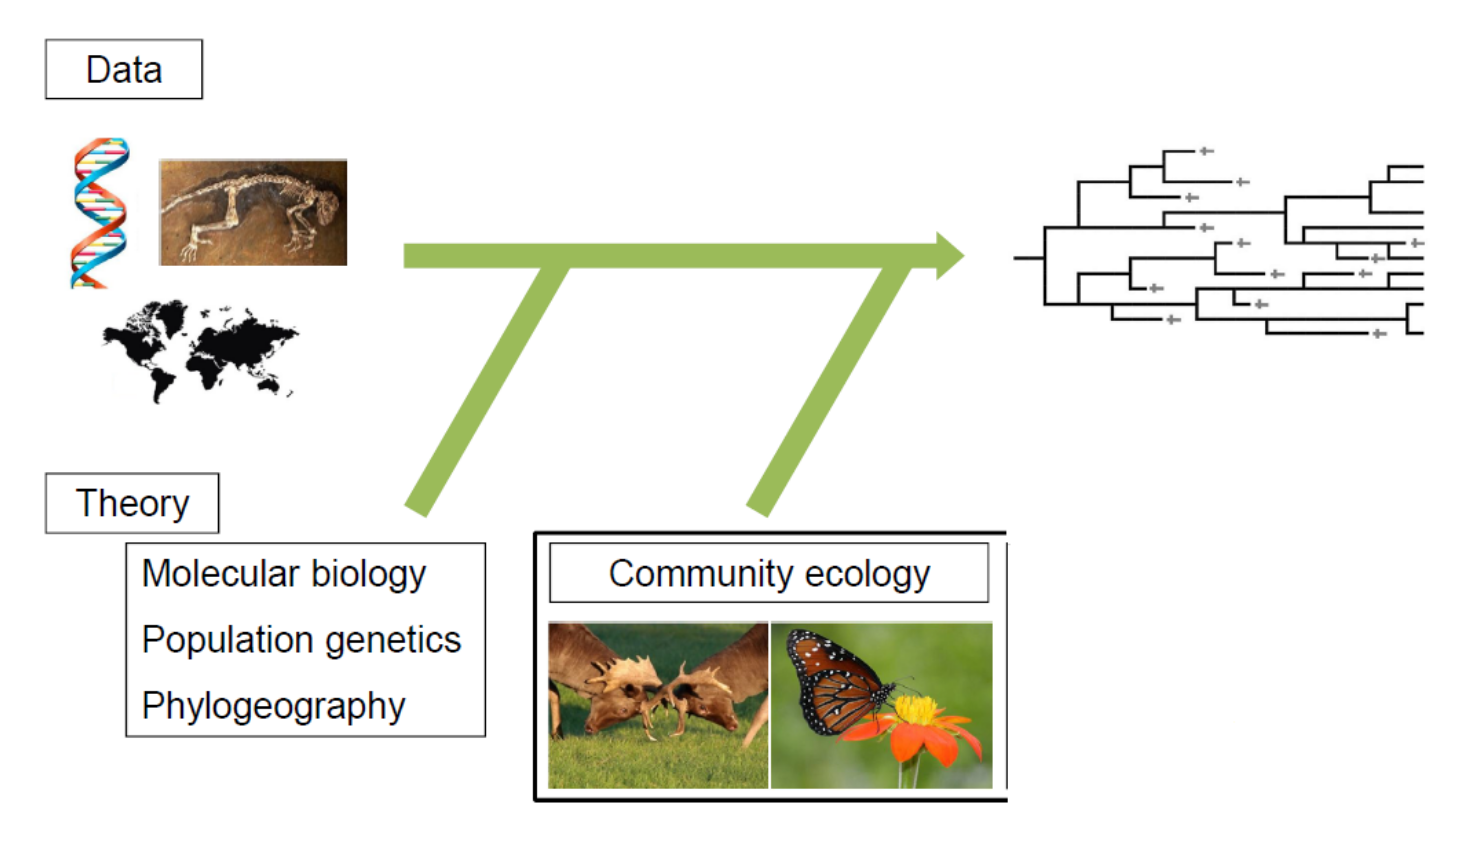
\includegraphics[width=.9\linewidth]{figures/datatree.png}
		\end{figure}   
          
The phylogenetic tree is mathematically determined by

\begin{itemize}
	\item A set of branching times $\mathcal{T}$% = \{t_1,t_2,...,t_n\}$.
	\item The topology  $\Upsilon$.% = \{ \mathfrak{S}, \mathfrak{X} \}$.   
\end{itemize}

And its likelihood function is defined as 

	\begin{equation} L( Y | \Theta) = \displaystyle\prod_{i=1}^p \sigma_i e^{-\sigma_i t_i} \frac{\rho_{i}}{\sigma_i}  
 		\label{llik}
 		\end{equation}
 		
	
Where $\sigma_i = \sum_{j=1}^{n_i} \lambda_{i,j} +\mu_{i,j} $; $\lambda_{i,j}$ is defined as the {\bf speciation rate} of the species $j$ at time $t_i$ and $\mu_{i,j}$ corresponds to the {\bf extinction rate} of the same species. $\rho_i \in \Upsilon$ is the topology variable corresponding to the speciation or extinction rate taking place on waiting time $t_i$. \\
Both $\lambda$ and $\mu$ are linear functions of many potential explanatory variables.
%

          \end{block}     
%          \begin{table}[ht]
%					\centering
%					\begin{tabular}{lccc}
%                    Patient Characteristics & n 		& & \%  \\
%					\hline
%					Total of Patients 		& 100     	& & 100 \\
%					Age 	 				&  45      	& &  45 \\
%					Gender 					&  50 	   	& &  50 \\
%				    \hline
%				  \end{tabular}
%				\caption{Considered scenarios} 
%                \label{Patient and tumor Characteristics}
%			  \end{table}
                \end{column}
                  
                  
                  
         \begin{column}{\sepwid}  \end{column}
         
         
         
         
         \begin{column}{\onecolwid} %The second column
          
     \begin{block}{Challenges}
     
     %In spite of the elegance of this general model, the accurate estimation of parameters is not posible in a straightfoward way due to two main reasons: 
     
     \begin{itemize}
     
     \item Decay and fossilization degrade crucial evidence useful for phylogenetic analyses that could infer underlying mechanisms. In fact, we normally observe extant species only.

	
\begin{figure}
                    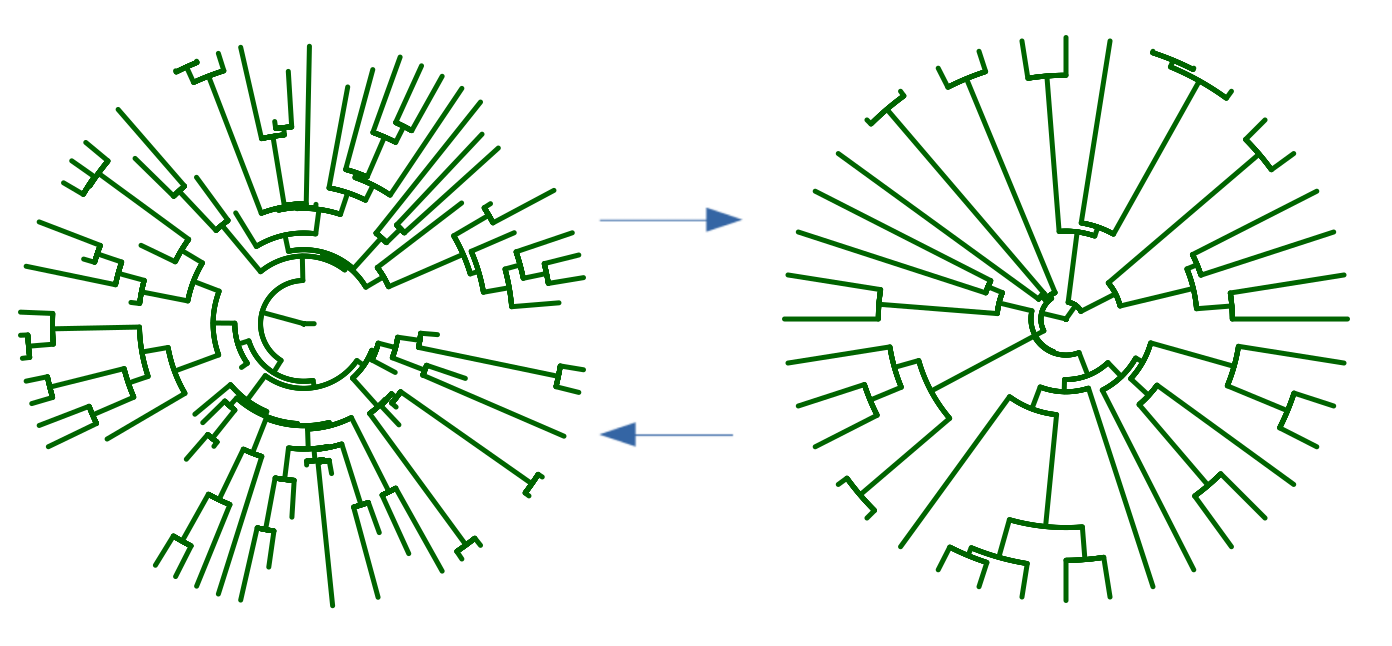
\includegraphics[width=1\linewidth]{figures/treesa2.png}
                    \caption{Phylogenetic trees where we can visualize the loss of information on reconstructed trees. At the left we have a tree with all extinct species whereas the right plot shows the same tree with only observable species.}
				\end{figure}
     
   \item Diversification processes have many potential explanatory variables, which increases the dimensionality and the complexity of current models enormously. 
     
     \end{itemize}
     
      \begin{figure}
                	%\vspace*{-1cm}
                    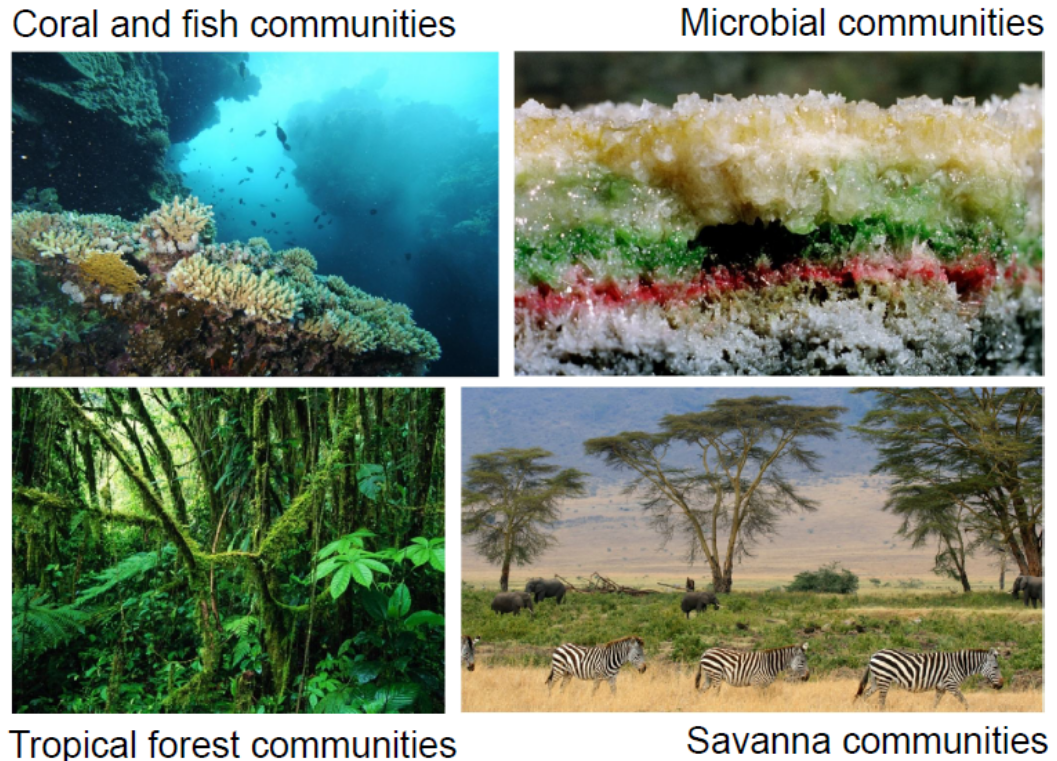
\includegraphics[width=1\linewidth]{figures/communities.png}
		\end{figure}
     
      \end{block}
   
   \end{column}
    \end{columns} 
       
      \begin{columns}[t] 
    \begin{column}{\twocolwid}
    \begin{block}{MCEM \& Case studies (work in progress)}
		The fact that we typically only have data on currently existing species is described as a missing data problem. Thus, we perform an MCEM algorithm 
     %  \[  Q(\theta | \tikzmark{a}{\theta_{(i)}}) = E[logL(\theta)|Y] = \bigint\limits_{\{ {\small \Springtree, \Autumntree, \Summertree,...} \}} logL(\theta|\Wintertree) d\Wintertree \longrightarrow \theta_{(i+1)}\tikzmark{b} = \displaystyle\argmax_{\theta} Q(\theta | \theta_{(i)} ) \] 
          
\[
Q(\theta | \textcolor{red}{\theta_{(i\tikzmark{a})}})% <-- changed
    = \smashoperator[r]{\bigint_{\{\small
                           \Springtree, \Autumntree, \Summertree, \dots \}}
                        }
    \log L(\theta|\Wintertree) \mathrm{d}\Wintertree \longrightarrow
           \textcolor{red}{\theta_{(i\tikzmark{b}+1)}}% <-- changed
    = \displaystyle\argmax_{\theta} Q\left(\theta | \theta_{(i)}\right)
\]


    \tikz[overlay,remember picture]
  % {\draw[->,square arrow] (b.south) to (a.south);}
{\draw[loop arrow] (b.south) to  (a.south);}% <-- changed   
    %      Let $X$ be the observed (extant species) tree and $Z$ the missing data (extinct species). Then the complete tree (unavailable) would be $Y = X \cup Z$. \\ 
          
  %        To compute the EM algorithm in this case we perform\\
     % \begin{subequations}    
      %   \begin{align*} 
       %   	(E) & \qquad  Q(\theta | \theta_{(i)}) = E_{\myleaf,\theta{(i)}}[l(\mytree|\theta)|X]  \\
        %  	(M) & \qquad \Wintertree \Springtree \Autumntree \Summertree \theta_{(i=1)} = \displaystyle\argmax_{\theta} Q(\theta | \theta_{(i)} )
		%\end{align*}
      %\end{subequations}          
          

          
          \end{block}		
		
	%	\begin{block}{Preliminary results: Diversity-dependence model}
		
%		\end{block}   
   \end{column}
    \end{columns} 
       
      \begin{columns}[t] 
      \hspace*{-2.9cm}
     \begin{column}{0.15\paperwidth}   
   \begin{block}{{\small Diversity-dependence}}
For the first case studies we plug in the diversity-dependence model \cite{etienne2011diversity} under the framework:  
   
  $$\begin{cases} \lambda_{i,j} = \lambda_0 + (\lambda_0 -\mu_0) \frac{N_i}{K}
   \\
	\mu_{i,j} = \mu_0    
     \end{cases}$$
 

   \end{block}
         

      \end{column}
         \begin{column}{0.28\paperwidth}   
   \begin{block}{{\small Case study 1: Dendroica}}
  
    \begin{minipage}{\textwidth}
   
   \begin{minipage}[b]{0.49\textwidth}
    \centering
    \tabcolsep=0.11cm
    {\footnotesize
    \begin{tabular}{lccc}
  \hline
EM iter & $\lambda_0$ & $K$ & $\mu_0$ \\ 
  \hline
1 & 4.00 & 30 & 1.00 \\ 
  2 & 1.51 & 36 & 0.77 \\ 
  3 & 0.97 & 116 & 0.61 \\ 
  4 & 0.88 & 811 & 0.56 \\ 
  5 & 0.85 & 3165 & 0.53 \\ 
  6 & 0.85 & \infty & 0.52 \\ 
  7 & 0.85 & \infty & 0.52 \\ 
   \hline
\end{tabular}
      \captionof{table}{MCEM iterations for Dentroica phylogeny.}   }
    \end{minipage}
     \hfill
  \begin{minipage}[b]{0.49\textwidth}
    \centering
    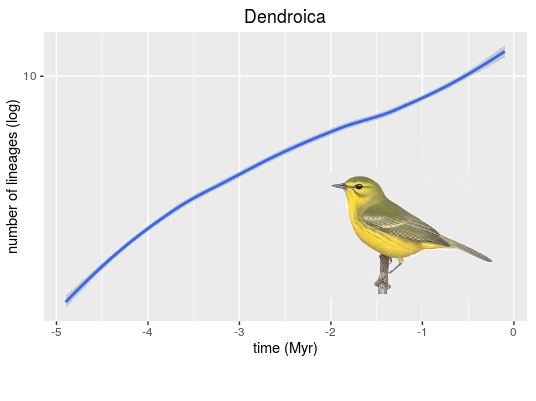
\includegraphics[width=1.1\linewidth]{figures/dend5.png}
    \captionof{figure}{Expectation of lineages through time for the obtained parameters}
  \end{minipage}
  \end{minipage}

   \end{block}
         

      \end{column}
      
     \begin{column}{0.28\paperwidth}   
   \begin{block}{{\small Case study 2: Foraminifera}}
  
    \begin{minipage}{\textwidth}
   
   \begin{minipage}[b]{0.49\textwidth}
    \centering
    \tabcolsep=0.21cm
    {\footnotesize
   \begin{tabular}{lccc}
  \hline
EM iter & $\lambda_0$ & $K$ & $\mu_0$ \\ 
  \hline
1 & 4.00 & 30 & 1.00 \\ 
  2 & 0.79 & 35 & 0.30 \\ 
  3 & 0.37 & 42 & 0.13 \\ 
  4 & 0.25 & 47 & 0.07 \\ 
  5 & 0.19 & 46 & 0.05 \\ 
  6 & 0.19 & 46 & 0.04 \\ 
  7 & 0.16 & 45 & 0.03 \\ 
  8 & 0.16 & 45 & 0.03 \\ 
%  9 & 0.16 & 43.60 & 0.03 \\ 
   \hline
\end{tabular} }
      \captionof{table}{MCEM iterations for Foraminifera phylogeny.}
    \end{minipage}
    % \hfill
  \begin{minipage}[b]{0.49\textwidth}
    \centering
    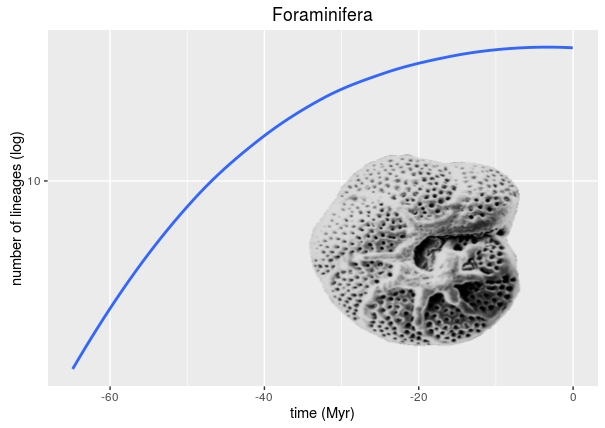
\includegraphics[width=1.12\linewidth]{figures/foraminifera2.png}
    \captionof{figure}{Expectation of lineages through time for the obtained parameters}
  \end{minipage}
  \end{minipage}

   \end{block}
         

      \end{column}      
      
    %  \begin{column}{\sepmargin} \end{column}
      \end{columns} 
       
      \begin{columns}[t] % Split up the two columns wide column again
      
      \begin{column}{\sepmargin} \end{column}
        \begin{column}{\onecolwid} % The first column
			%\begin{block}{\large Acknowledgements}
             %       \begin{center}
				%		\begin{tabular}{SL}
				%			
\includegraphics[width=\linewidth]{Flag_of_Europe.png}  &
				%			\footnotesize This project has received funding from the  grant agreement No 11111.
				%		\end{tabular}
				%	\end{center}
			%	\end{block}	
                \vspace*{-0.9cm}
				\begin{alertblock}{\large Contact Information}
                \vspace*{-0.5cm}
					\begin{footnotesize}
					\begin{itemize}
						\item \href{mailto:f.richter@rug.nl}{f.richter@rug.nl}
						%\item \href{http://www.example.com/}{www.example.com} -
						%\item \href{https://nl.linkedin.com/in/franciscorichter}{https://nl.linkedin.com/in/franciscorichter}
					\end{itemize}
					\end{footnotesize}	
					
				\end{alertblock}
		    \end{column} % End of the first column
			\begin{column}{\sepwid}\end{column} % Empty spacer column
			\begin{column}{\onecolwid} % Begin a column 
              \begin{block}{\large References}
			  \vspace*{-0.5cm}
              	\nocite{*} % Insert publications even if they are not cited in the poster
					{\footnotesize
                    	%\bibliographystyle{plainurl}
						\bibliography{bibliog.bib}}
				\end{block} 
			\end{column} % End of the second column
            
			\begin{column}{\sepmargin}\end{column} % Empty spacer column
            
\end{columns} % End of all the columns in the poster


\end{frame} % End of the enclosing frame
	
\end{document}